\documentclass[11pt]{standalone}

\usepackage{helvet}

\usepackage{ifthen}
\usepackage{tikz} 
\usetikzlibrary{shapes.misc}
\usetikzlibrary{arrows,arrows.meta}
\usetikzlibrary{calc,intersections, patterns, math}

\definecolor{pfeil}{RGB}{168,167,167}
\definecolor{petrol}{RGB}{0, 118, 136}
\definecolor{darkgoldenrod}{RGB}{184, 134, 11}
\colorlet{petrol-lighter}{petrol!40}
\colorlet{darkgoldenrod-lighter}{darkgoldenrod!40}

\begin{document}

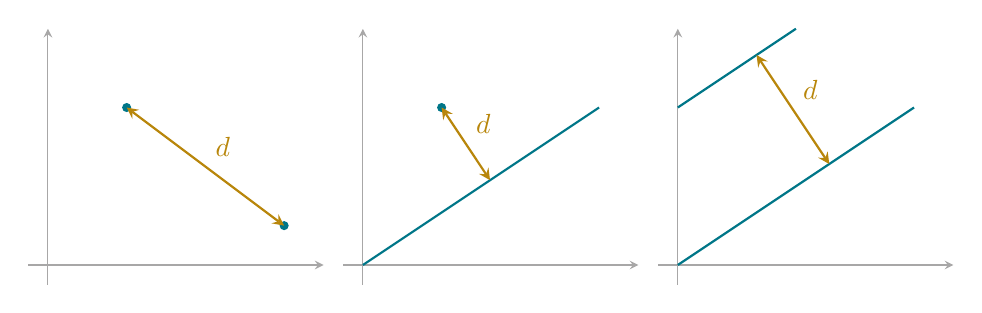
\begin{tikzpicture}[pfeil]

    % \draw[thick, fill=petrol!20, draw=petrol-lighter, rounded corners=2ex, opacity=0.5] (0,0) rectangle ++ (1.5,3.5);
    % \draw[thick, fill=darkgoldenrod!20, draw=darkgoldenrod-lighter, rounded corners=2ex, opacity=0.5] (5,0) rectangle ++ (1.5,3.5);

    \draw[-stealth] (-0.25,0) -- (3.5,0);
    \draw[-stealth] (0,-0.25) -- (0,3);

    \draw[petrol, fill] (1,2) circle (0.05);
    \draw[petrol, fill] (3,0.5) circle (0.05);
    \draw[thick, darkgoldenrod, stealth-stealth] (1,2) -- node[above right] {$d$} (3,0.5);

    \begin{scope}[shift={(4,0)}]
        \draw[-stealth] (-0.25,0) -- (3.5,0);
        \draw[-stealth] (0,-0.25) -- (0,3);

        \draw[petrol, fill] (1,2) circle (0.05);
        \draw[petrol, thick] (0,0) -- (3,2);
        \draw[thick, darkgoldenrod, stealth-stealth] (1,2) -- node[above right] {$d$} (1.615,1.077);
    \end{scope}


    \begin{scope}[shift={(8,0)}]
        \draw[-stealth] (-0.25,0) -- (3.5,0);
        \draw[-stealth] (0,-0.25) -- (0,3);

        \draw[petrol, thick] (0,2) -- (1.5,3);
        \draw[petrol, thick] (0,0) -- (3,2);
        \draw[thick, darkgoldenrod, stealth-stealth] (1,2.667) -- node[above right] {$d$} (1.923,1.282);
    \end{scope}


\end{tikzpicture}

\end{document}
